\chapter{Sentiment Analysis}
	????????????
	
	\section{Richiami teorici}
		L'analisi del \textit{sentiment} o \textit{sentiment} \textit{analysis} (nota anche come \textit{opinion} \textit{mining}) è un campo dell'elaborazione del linguaggio naturale che si occupa di costruire sistemi per l'identificazione ed estrazione di opinioni dal testo, basandosi sui principali metodi di linguistica computazionale e di analisi testuale. Per identificare le informazioni soggettive che denotano opinioni , è necessario determinare la polarità insita in esse. Questa può essere di tre tipi: positiva, negativa o neutra.
		
		\begin{description}
			\item [polarità positiva:] l'informazione che ricaviamo è positiva.
			\item [polarità negativa:] l'informazione che ricaviamo è negativa.
			\item [polarità neutra:] non ricaviamo alcuna informazione sulla polarità. Questo può avvenire per due diversi motivi:
			
			\begin{itemize}
				\item le opinioni positive sono bilanciate da quelle negative;
				\item non si manifesta alcun sentimento.
			\end{itemize}
			
		\end{description}
	
		Per il calcolo della polarità esistono diversi tipi di approccio: basato sul lessico, supervisionato, semi-supervisionato e non supervisionato.
		
		\begin{description}
			\item [Approccio basato sul lessico:] la polarità viene calcolata analizzando la frase.
			\item [Approccio supervisionato:] la polarità viene calcolata utilizzando le tecniche del \textit{Machine Learning}. Inserisco prima le parole in cui la polarità è esplicita, poi aggiungo le altre per fare inferenza.
			\item [Approccio semi-supervisionato:] ????????
			\item [Approccio non supervisionato:] ????????	
		\end{description}
		
		Vedremo che per il nostro non è stato necessario andare a calcolare il \textit{sentiment}; in quanto un attributo si prestava bene per questo tipo di analisi.
		
	\section{Textual Preprocessing}
		Il nostro primo obiettivo è quello di studiare l'intrattenimento, in particolare quali siano i prodotti più recensiti all'interno delle nostre quattro categorie. Abbiamo scelto di effettuare lo studio su un numero limitato di prodotti, riducendoli a duecento, e di analizzare la loro distribuzione in questo sottoinsieme. I risultati ottenuti sono presentati nella Figura \ref{fig:pie_category}
		
		\begin{figure} [h]
			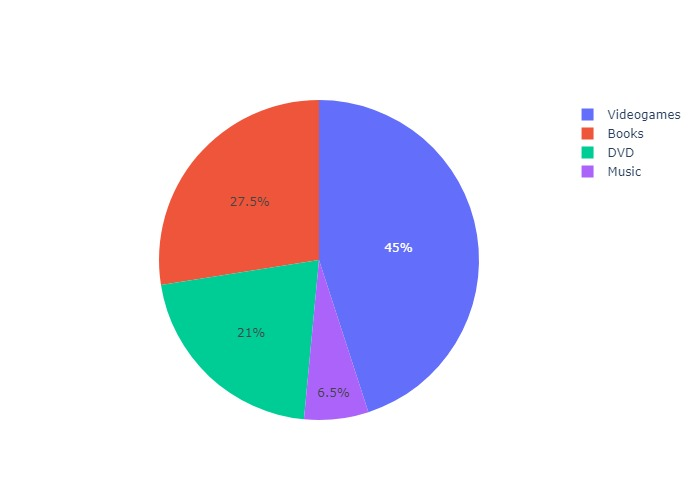
\includegraphics[width=\textwidth]{Figure/pie_category}
			\caption{\textit{Distribuzione delle recensioni per ogni categoria}.}
			\label{fig:pie_category}
		\end{figure}
	
		Per poter eseguire delle analisi consistenti sono indispensabili una serie di operazioni atti a uniformare il \textit{dataset}. Con il termine "uniformare" intendiamo riscrivere i dati seguendo delle specifiche regole comuni. Nel seguito ogni procedura verrà descritta nel dettaglio.
		
		
		